%%%%%%%%%%%%%%%%%%%%%%%%%%%%%%%%%%%%%%%%%
%
% (c) 2018 by Jennifer Laaser
%
% This work is licensed under the Creative Commons Attribution-NonCommercial-ShareAlike 4.0 International License. To view a copy of this license, visit http://creativecommons.org/licenses/by-nc-sa/4.0/ or send a letter to Creative Commons, PO Box 1866, Mountain View, CA 94042, USA.
%
% The current source for these materials is accessible on Github: https://github.com/jlaaser/quantum-exercises
%
%%%%%%%%%%%%%%%%%%%%%%%%%%%%%%%%%%%%%%%%%

\section*{The Helium Atom\sectionmark{Exercise: The Helium Atom}}

	\begin{questions}
	
		\question The ``helium-like'' atom, diagrammed below, is just like a ``hydrogen-like'' atom, but has two electrons rather than one:
		
			%\begin{minipage}{0.55\textwidth}
				\centerline{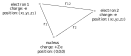
\includegraphics[width=0.5\textwidth]{includes/the-He-atom-FIGURES/He-atom}}
			%\end{minipage}
		
			\begin{parts}
				\part Assuming the nucleus is fixed in place (i.e. can't move), what is the \emph{kinetic} energy for the helium-like atom?  (You may use the $\nabla^2$ notation for the Laplacian(s); just put appropriate subscript(s) on it to indicate which set(s) of coordinates it refers to.)
				
					\begin{solution}[1.75in]
					\end{solution}				
				
				\part What is the \emph{potential} energy for this system?  Remember that the electrostatic energy of interaction between particles of charge $Q_1$ and $Q_2$ separated by distance $r$ is $\frac{Q_1Q_2}{4\pi\epsilon_0 r}$.
				
					\begin{solution}[1.75in]
					\end{solution}
				
				\part What is the \emph{Hamiltonian} for this system?
				
					\begin{solution}[1.5in]
					\end{solution}
				
				\contdnewpg
				\part The Hamiltonian you wrote (or should have written!) in part (c) is not separable.  Why? Which term causes the problem?
				
					\begin{solution}[2in]
					\end{solution}
				
				\part If you could ignore the ``problem'' term, what form do you think the wavefunction would take? You may write your answer out in words if you'd like; we'll formalize the notation together as a class.
				
					\begin{solution}[2.5in]
					\end{solution}
				
				\part If you calculated an expectation value for the energy using this simplified wavefunction and the full Hamiltonian, do you think the answer would over- or under-estimate the true ground-state energy?  Why?
				
					\begin{solution}[2.25in]
					\end{solution}
			\end{parts}
	\end{questions}
	
\stophere